\section{Systemy jednoukładowe}

\subsection{Wprowadzenie do komputerów jednopłytkowych}

Komputery jednopłytkowe, których istnienie zawdzięczyć można postępowi miniaturyzacji układów scalonych, to systemy komputerowe, które zawierają całą wymaganą funkcjonalność na pojedynczej płytce drukowanej. Od typowego systemu komputerowego różni je to, że zwykle nie posiadają gniazd rozszerzeń, które byłyby wykorzystywane do rozbudowania komputera o dodatkowe lub czasami nawet wymagane rozszerzenia, które byłyby potrzebne w wybranym zastosowaniu danego systemu komputerowego. Pozwala to na zredukowanie ceny kosztem ograniczonych możliwości rozbudowy komputera.

Pierwsze komputery jednopłytkowe powstały w latach 70-tych\cite{Ariza_2021}, często w formie zestawu do samodzielnego złożenia i uruchomienia. Były one tańszą alternatywą dla większych systemów komputerowych, oferując podstawowe peryferia wymagane do tworzenia oprogramowania i interakcji z nim.
W późniejszych czasach komputery jednopłytkowe były coraz częściej wykorzystywane w systemach przemysłowych, głównie z powodu większej integracji komponentów i większej wytrzymałości niż systemy złożone z większej ilości elementów takich jak karty rozszerzeń.

Po upowszechnieniu się standardów takich jak IBM PC\cite{ibmpc1981}, część komputerów jednopłytkowych powstających w późniejszym czasie zaczęły wykorzystywać komponenty takie jak procesory architektury x86. Umożliwiło to wytwarzanie i uruchamianie programów oryginalnie przeznaczonych dla komputerów zgodnych z tymi standardami. Obecnie jednak, ze względu między innymi na mniejsze zużycie prądu, najczęściej wykorzystuje się układy bazujące na procesorach architektury ARM, znanej z urządzeń mobilnych.

Obecnie komputery jednopłytkowe większość funkcjonalności mają zawarte w pojedynczym układzie, zwanym System on Chip (system jednoukładowy). Poprzez redukcję ilości elementów na płytce drukowanej możliwym było zredukowanie rozmiarów komputerów jednopłytkowych, czasami zbliżając się rozmiarami do karty bankowej.

Przykładami popularnych obecnie komputerów jednopłytkowych, zbudowanych z użyciem układów SoC, są:
\begin{itemize}
	\item Raspberry Pi\cite{rpi1bplus} (Raspberry Pi Trading, Ltd.),
	\item BeagleBoard\cite{beagleboard} (Texas Instruments, BeagleBoard.org Foundation),
	\item UDOO Bolt\cite{udoobolt} (SECO S.P.A.)
\end{itemize}

\todo[inline]{ZDJĘCIE: popularny komputer jednopłytkowy}

\subsection{Definicja układu System on Chip w porównaniu z mikrokontrolerem}

Układy typu System on Chip (SoC) to układy, które na jednym podłożu półprzewodnikowym integrują wszystkie komponenty składające się na kompletny system mikroprocesorowy. Dzięki wysokiemu stopniu integracji układy te pozwoliły na znaczną miniaturyzację urządzeń elektronicznych bazujących na systemach mikroprocesorowych, takich jak telefony komórkowe czy komputery przenośne, oraz na ograniczenie kosztów przy większej skali produkcji.

Pojedynczy układ SoC składa się z przynajmniej jednej jednostki centralnej, pamięci RAM i ROM pozwalających na uruchomienie kodu inicjalizującego układ, peryferiów pozwalających na komunikowanie się ze światem zewnętrznym oraz jednej lub więcej magistral, które łączą wcześniej wspomniane peryferia.

Układy SoC odróżniają się od mikrokontrolerów tym, iż zawierają w sobie jak największą funkcjonalność możliwą do zmieszczenia w określonym rozmiarze fizycznym, uwzględniając takie ograniczenia jak dostępny proces technologiczny czy pobór prądu. Mikrokontrolery za to posiadają ograniczoną ilość peryferiów oraz mocy obliczeniowej w celu redukcji kosztów, co jest ważne w przypadku urządzeń wymagających specyficznej funkcjonalności w ograniczonym budżecie.

\begin{figure}[H]
\centering
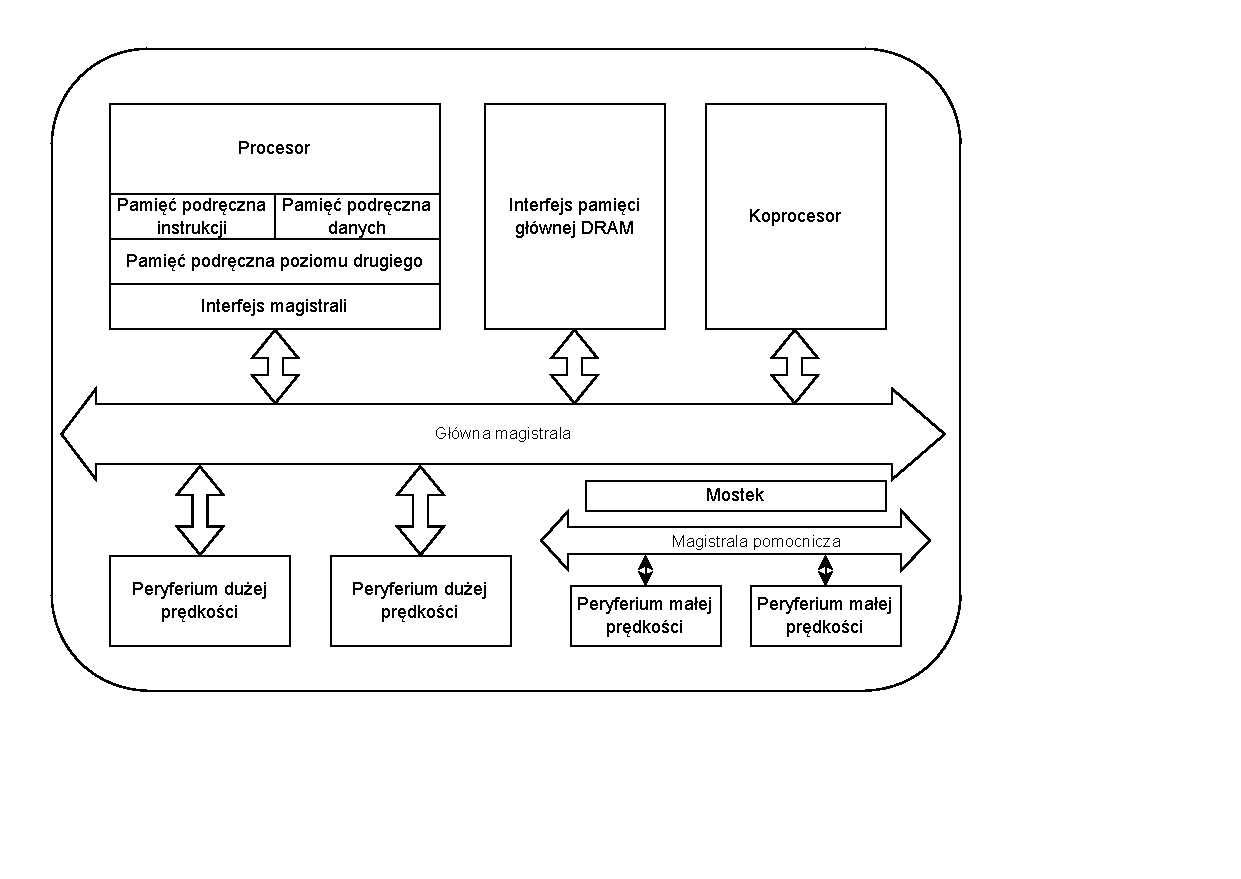
\includegraphics[scale=0.7,trim={0 3cm 3cm 0.3cm},clip]{soc-theory/diag-soc-schem.pdf}
\caption{Uproszczony schemat typowego układu System on Chip}
\label{fig:soc-schem}
\end{figure}

Na rysunku \ref{fig:soc-schem} przedstawiony został schemat przykładowego układu SoC. Posiada on przynajmniej jedną jednostkę centralną o stosunkowo dużej mocy obliczeniowej, która pozwala na uruchamianie pełnoprawnych systemów operacyjnych, takich jak Linux czy Microsoft Windows. Oprócz tego zaznaczony został kontroler DRAM, który odpowiada za komunikację z zewnętrzną pamięcią RAM. Pamięć ta nie jest zintegrowana w samym układzie SoC ze względu na ograniczone rozmiary układu oraz umożliwienie wybrania rozmiaru pamięci, jaka będzie wykorzystywana w danym systemie jednoukładowym. Procesor, interfejs pamięci głównej oraz pozostałe peryferia są połączone jedną lub większą ilością magistral, które odpowiadają za transfer danych między komponentami systemu. Mogą różnić się one takimi parametrami jak przepustowość lub szerokość linii danych, zaś dane między nimi są wymieniane z użyciem mostków.

Wśród różnych rodzin układów SoC, stosowanych w komputerach jednoukładowych, wymienić można:
\begin{itemize}
	\item OMAP\cite{omap3530} firmy Texas Instruments,
	\item Vortex86\cite{vortex86ex2} firmy DM\&P,
	\item JH71x0\cite{jh7110} firmy Shanghai StarFive Technology
\end{itemize}

\subsection{Opis wybranej implementacji procesora z ISA RISC-V}

Łatwa dostępność dokumentacji związanej z architekturą RISC-V spowodowała, że istnieje duża ilość projektów implementujących procesory z nią zgodne. Procesory te są w większości zoptymalizowane do uruchomienia na układach FPGA (Field Programmable Gate Array), różniąc się w większości wewnętrzną architekturą oraz udostępnioną funkcjonalnością.

Przykładowe projekty procesorów gotowych do wykorzystania w projektach bazujących na układach FPGA to:
\begin{itemize}
	\item PicoRV32\cite{picorv32} autorstwa Claire Wolf,
	\item Ibex\cite{ibex} od grupy lowRISC C.I.C.,
	\item rodzina OpenXuantie\cite{openxuantie} firmy T-Head Semiconductor
\end{itemize}

Na potrzeby tej pracy został wybrany projekt VexRiscv\cite{vexriscv:2018:Online}, który jest rdzeniem implementującym architekturę RISC-V\cite{Waterman:EECS-2014-54} w wariancie 32-bitowym (RV32I), zoptymalizowanym pod kątem układów FPGA. Jego modularność z użyciem rozszerzeń pozwala na konfigurację parametrów na etapie budowania rdzenia w zależności od wymogów projektu, takich jak ilość etapów potoku wykonywania rozkazów, wspierane rozszerzenia architektury czy wielkość pamięci podręcznej poziomu pierwszego.

Wśród dostępnych opcji konfiguracyjnych są takie elementy jak:
\begin{itemize}
	\item opcjonalne rozkazy m.in. mnożenia, operacji na liczbach zmiennoprzecinkowych zdefiniowanych dla architektury RISC-V,
	\item regulowana długość potoku wykonawczego od 2 do 5 stopni,
	\item możliwość podłączenia procesora do dowolnej magistrali, z czego dostępne są adaptery dla magistral AXI4, Avalon oraz Wishbone,
	\item opcjonalna pamięć podręczna programu i danych, każda w dowolnej ilości,
	\item opcjonalna jednostka zarządzania pamięcią (MMU)
\end{itemize}

Wybór tego procesora na potrzeby pracy został podyktowany przede wszystkim wcześniejszym doświadczeniem autora niniejszej pracy w pracy z tym projektem. Na potrzeby tej pracy użyta zostanie podstawowa konfiguracja. Ze względu na możliwe ograniczenia związane z platformą testową (na przykład rozmiar układu FPGA), wyłączone zostało wsparcie dla wszystkich opcjonalnych grup rozkazów. W zamian dodana zostanie pamięć podręczna danych, która odpowiedzialna będzie za buforowanie odczytywanych z potencjalnie wolniejszej pamięci operacyjnej danych.

\subsection{Przegląd dostępnych magistrali systemowych}

Magistrale, jak zostało wspomniane w poprzednich podrozdziałach, służą do transferu danych między poszczególnymi komponentami systemu. Od ich parametrów zależy sprawność komunikacji między peryferiami - źle skonfigurowana magistrala może spowalniać działanie całego systemu, przykładowo poprzez ograniczenie przepływności danych.

W celu wykorzystania danej szyny, wszystkie komponenty muszą mieć zaimplementowany interfejs, który pozwala na podłączenie się do danej magistrali. Jeśli któreś komponenty implementują interfejs innego mostka niż pozostałe, to można wykorzystać mostki, które pozwalają na konwersję między danymi standardami magistral.

Istnieją różne standardy magistrali przeznaczone dla układów SoC, wśród których bardziej znanymi standardami są:
\begin{itemize}
	\item AMBA AXI\cite{amba-axi:2021:Online} od Arm Ltd.,
	\item Avalon\cite{avalon:2005:Online} autorstwa firmy Altera,
	\item Wishbone\cite{wishbone:2019:Online} od Silicore Corporation
\end{itemize}

Każda z tych specyfikacji ma swoje unikalne cechy: przykładowo AMBA AXI definiuje niezależne kanały do odczytu i zapisu danych, pozwalając na jednoczesne wykonywanie tych dwóch operacji. Wishbone zaś definiuje wyłącznie sposób przekazywania danych między dwiema modułami, pomijając między innymi kwestię topologii połączeń między elementami.

W ramach tej pracy wykorzystywana będzie magistrala Wishbone ze względu na w pełni dostępną publicznie, wolną od tantiemów specyfikację oraz jej neutralność (nie została stworzona przez dużego producenta mikroprocesorów czy układów FPGA).

\subsection{Wnioski}

Jako, iż celem tej pracy jest poprawa wydajności systemu jednoukładowego, na początek wymagane było zdefiniowanie, czym ów system jest z uwzględnieniem tła historycznego oraz jaka jest typowa konstrukcja takiego układu. Po określeniu najważniejszych elementów takiego systemu dobrane zostały główne elementy, które będą wykorzystywane w niniejszej pracy: procesor VexRiscv, obsługujący rozkazy architektury RISC-V, oraz magistrala Wishbone, która definiować będzie sposób komunikacji między poszczególnymi elementami układu SoC.
